





\documentclass{nature}
\usepackage{amsmath}
\usepackage{amssymb}
\usepackage{eurosym}
\usepackage{graphicx}
\makeatletter
\let\saved@includegraphics\includegraphics
\AtBeginDocument{\let\includegraphics\saved@includegraphics}
\renewenvironment*{figure}{\@float{figure}}{\end@float}
\makeatother








\usepackage{url} %
\usepackage[hyperpageref]{backref} %
\usepackage[pagebackref]{hyperref}
\hypersetup{
  colorlinks=true, %
  urlcolor=purple,    %
  linkcolor=blue,  %
  citecolor=violet,   %
}
\usepackage{bm}
\usepackage{indentfirst}
\usepackage{tocbibind}
\usepackage{amsmath}
\usepackage{tcolorbox}
\usepackage{amssymb}
\usepackage{eurosym}
\usepackage{amsfonts}
\usepackage{enumerate}
\usepackage{babel}
\usepackage{graphicx}
\usepackage{caption}
\usepackage{supertabular}
\usepackage{tabularx}
\usepackage{float}
\usepackage{dsfont}
\usepackage{fancyvrb}
\usepackage{verbatim}
\usepackage{enumitem}
\usepackage{comment}
\usepackage{subcaption}
\usepackage{tikz}
\usepackage{gensymb}
\usepackage{textcomp}

\usepackage{tabulary}
\usepackage{tabularx}
\usepackage{booktabs}
\usepackage{fullpage}
\usepackage{morefloats}
\usepackage{makecell}
\usepackage{lscape}
\usepackage{pdflscape}
\usepackage{longtable}
\usepackage{rotating}
\usepackage{fancyhdr}
\usepackage{tocloft}
\usepackage{titletoc}
\usepackage[export]{adjustbox}
\usepackage[anythingbreaks]{breakurl} %
\usepackage{multicol}
\newsavebox\ltmcbox %
\renewcommand{\floatpagefraction}{.99}
\newenvironment{stretchpars}{\par\setlength{\parfillskip}{0pt}}{\par} %

\makeatletter
\newcommand{\fakesection}[1]{%
  %
  \par\nopagebreak
  %
  \refstepcounter{section}
  %
  \def\@currentlabelname{#1}
  %
  \addcontentsline{toc}{section}{\protect\numberline{\thesection}#1}
}
\makeatother










\title{International Attitudes Toward Global Policies %
} 

\author{Adrien Fabre$^{1,2}$, Thomas Douenne$^3$ and Linus Mattauch$^{4,5,6}$} %


\begin{document}

\maketitle

\begin{center}
\end{center}


\begin{affiliations}
\item Centre National de la Recherche Scientifique
\item Centre International de Recherches sur l'Environnement et le Développement
\item University of Amsterdam
\item Technical University Berlin
\item Potsdam Institute for Climate Impact Research 
\item University of Oxford
\end{affiliations}

\begin{abstract}
  %

  Major sustainability objectives could be achieved by global approaches to mitigating climate change and inequality. For instance, a global carbon price funding a global basic income, called the ``Global Climate Scheme'' (GCS), would be an effective way to jointly combat climate change and poverty. %
  Yet, few prior attitudinal surveys have examined support for global policies. To explore relevant public attitudes, we survey %
  %
  %
  %
  over 48,000 respondents from 20 high- and middle-income countries. %
  We find that there exists substantial support for global policies addressing climate change and global inequality, even in high-income countries. The GCS is supported by three quarters of Europeans and half of Americans. 
  Further responses reveal strong support for global redistributive policies, including the GCS and a global wealth tax aimed at financing low-income countries. We test whether support of the expressed preference is sincere: a list experiment shows no evidence of social desirability bias in survey responses, majorities are willing to sign a real-stake petition, and global redistribution ranks high in the prioritization of policies. Conjoint analyses reveal that a political platform is more likely to be preferred if it contains the GCS or a global tax on millionaires. In sum, our findings indicate that global redistributive policies are genuinely supported by a majority of the population, even in wealthy nations that would bear a significant burden. %
  %
\end{abstract}








Major sustainability objectives could be achieved by global approaches to mitigating climate change and poverty.\cite{budolfson_climate_2021,franks_mobilizing_2018,dennig_inequality_2015,soergel_combining_2021} For example, an equal per capita dividend paid out of 2 degree compatible carbon prices can improve well-being as well as reduce inequality and poverty at a national level.\cite{budolfson_climate_2021} Global carbon pricing is even more redistributive.\cite{bauer_quantification_2020} 
However, disagreements on burden-sharing, differing priorities, and lack of institutional capacity are commonly seen as obstacles to effective global collaboration on these objectives.\cite{cramton_global_2017} We examine a key condition for the success of global cooperation, neglected in social science research so far: the support of citizens in affluent countries for globally redistributive policies.%

Recent surveys administered to over 40,000 respondents from 20 high- and middle-income countries reveal substantial support for those policies, especially global climate policies and a global tax on the wealthiest aimed at financing low-income countries %
(other questions from these surveys are analyzed in a companion paper\cite{dechezlepretre_fighting_2022}). %
 
In particular, a global 2\% tax on individual wealth in excess of \$5 million would effectively reduce poverty as it would, to first order, increase low-income countries' national income by 50\%, if merely 35\% of the revenue were allocated for this purpose.\cite{chancel_world_2022} %
Surprisingly, even in wealthy nations that would bear a significant burden, majorities of citizens express support for such globally redistributive measures.%

To gain insights into the factors shaping public support for global policies in high-income countries, we conducted complementary surveys among 8,000 respondents from France, Germany, Spain, the U.S., and the UK. The focus of our approach is a specific policy aimed at addressing both climate change and poverty, referred to as the ``Global Climate Scheme'' (GCS). It implements a cap on carbon emissions to limit global warming below 2\textdegree{}C. The emission rights are auctioned each year to polluting firms and fund a global basic income, alleviating extreme poverty. Although the GCS may seem idealistic, we focus on this policy as its key features allow us to expose respondents in a concise and simple way with the key trade-off between the costs and benefits of globally redistributive climate policies. %
By employing a list experiment, a real-stake petition, and conjoint analyses, our study indicates genuine and robust support for the GCS among respondents. For example, the conjoint analyses provide evidence that political parties would not lose vote intention by endorsing the GCS.%


These findings underscore a strong demand for globally redistributive climate policies, even in the absence of significant policy proposal. In our discussion we offer potential explanations behind this policy implementation gap, indicating that public opinion does not seem to be the reason that they are rarely mentioned in public debates.












\paragraph{Literature} A wealth of studies have examined public support for national carbon pricing policies.\cite{kotchen_public_2017,klenert_making_2018,douenne_yellow_2022,dechezlepretre_fighting_2022} %
Yet, few prior attitudinal surveys have examined policies for global redistribution. They find agreement close to 50\% in high-income countries for global carbon taxes with international per capita redistribution;\cite{carattini_how_2019} and near consensus that ``present economic differences between rich and poor countries are too large'' (overall, 78\% agree and 5\% disagree) in each of 29 countries.\cite{issp_international_2019} Furthermore, correcting misperceptions concerning one's position in the world's income distribution does not affect the support for global redistributive policies.\cite{fehr_your_2022} Besides, an international study of the support for global democracy finds that, in countries governed by a coalition, voting shares would shift by 8 (Brazil) to 12 p.p. (Germany) from parties that are said to oppose global democracy to parties that supposedly support it.\cite{ghassim_public_2022} Supplementary Section A summarises attitudinal surveys on global policies; prior work on attitudes toward climate burden sharing, attitudes toward foreign aid; global carbon pricing, global redistribution, basic income, and global democracy.







\subsection{Data}\label{subsec:data}



The study relies on two sets of representative surveys. 
The %
\textit{Global} survey 
is tied to %
another paper, that focuses on attitudes toward climate change and national climate policies.\cite{dechezlepretre_fighting_2022} %
The \textit{Global} survey was conducted in 2021--2022 on 40,680 respondents from 20 countries covering 72\% of global CO$_\text{2}$ emissions. 
\textit{Complementary} surveys in the U.S. (\textit{US1}: N=3,000, \textit{US2}: N=2,000) and four European countries (\textit{Eu}: N=3,000) were conducted 
in 2023 (See \nameref{sec:methods} for details on data collection and data quality).%










\section{Stated support for global policies}\label{subsec:stated_support}


\paragraph{Global support}\label{subsubsec:global_support} %

The Global survey shows strong support for climate policies enacted at the global level (Figure \ref{fig:oecd}). %
When asked ``At which level(s) do you think public policies to tackle climate change need to be put in place?'', 70\% (in the U.S.) to 94\% (in Japan) choose the global level. The next most popular choice is the federal or continental level, favored by 52\% of U.S. and less than half of European respondents. Local policies receive the least support. 


\begin{figure}[h!]
  %
  \caption[Relative support for global climate policies]{Relative support for global climate policies (Reproduced from Dechezleprêtre et al. (2022),\cite{dechezlepretre_fighting_2022} Figure A21.).} %
  \makebox[\textwidth][c]{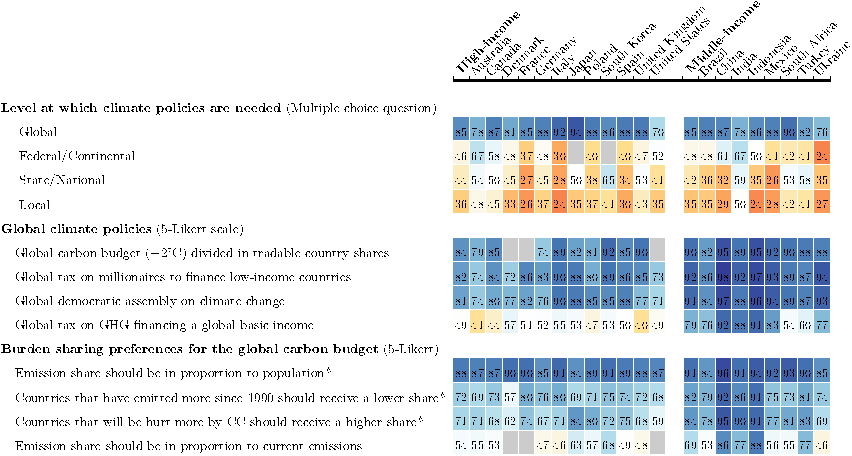
\includegraphics[width=1.2\textwidth]
  {../figures/OECD/Heatplot_global_tax_attitudes_share.pdf}}\label{fig:oecd} %
  {\footnotesize %
  Note 1: The numbers represent the share of \textit{Somewhat} or \textit{Strongly support} among non-\textit{indifferent} answers (in percent, $n$ = 40,680). The color blue denotes a relative majority. See Supplementary Figure A3 for the absolute support. (Questions A-I in Supplementary Section C).
  %
  \\ Note 2: *In Denmark, France and the U.S., the questions with an asterisk were asked differently, cf. Question F in Supplementary Section C.%
  } 
\end{figure}

Among the four global climate policies examined in the \textit{Global} survey, three policies garner high support across all countries (Figure \ref{fig:oecd}). These policies include a global democratic assembly on climate change, a global tax on millionaires to finance low-income countries contingent on their climate action, and a global carbon budget of +2\textdegree{}C divided among countries based on tradable shares. %
The three policies garner a majority of absolute support (i.e., ``somewhat'' or ``strong'' support) in all countries (except in the U.S. for the global assembly, 48\% absolute support). In high-income countries, the global quota policy obtains 64\% absolute support and 84\% relative support (i.e., excluding ``indifferent'' answers). 

Following the support for the global quota, respondents are asked about their preferences for dividing the carbon budget among countries, as depicted in the third block of Figure \ref{fig:oecd}. Consistent with the existing literature (see Supplementary Section A.1.2), an equal per capita allocation of emission rights emerges as the preferred burden-sharing principle, garnering absolute majority support in all countries and never below 84\% relative support. Taking into account historical responsibilities or vulnerability to climate damages is also popular, albeit with less consensus, while grandfathering (i.e., allocation of emission shares in proportion to current emissions) receives the least support in all countries.

A global quota with equal per capita emission rights produces the same distributional outcomes as a global carbon tax that funds a global basic income. %
The support for the global carbon tax is also tested and its redistributive effects --  the average increase in expenditures along with the amount of the basic income -- are specified to the respondents explicitly (see box below). %
The support for the carbon tax is lower than for the quota, particularly in high-income countries, and there is no relative majority for the tax in Anglo-Saxon countries. %
Two possible reasons for this lower support are that distributive effects are made salient in the case of the tax, and that citizens may find a quota more effective than a tax to reduce emissions. This interpretation is consistent with the level of support for the global quota once we make the distributive effects salient, as we do in the complementary surveys.




\paragraph{Global Climate Scheme}\label{subsubsec:support_gcs} %

The complementary surveys (\textit{US1}, \textit{US2}, \textit{Eu}) consist of a comprehensive exploration of citizens' attitudes toward the GCS. We present to respondents a detailed description of the GCS and explain its distributive effects, including specific amounts at stake (as specified in the box below). 
Furthermore, we assess respondents' understanding of the GCS with incentivized questions to test their comprehension of the expected financial outcome for typical individuals in high-income countries (loss) and the poorest individuals globally (gain), followed by the provision of correct answers. The same approach is applied to a National Redistribution scheme (NR) targeting the top 5\% (in the U.S.) or top 1\% (in Europe) with the aim of financing cash transfers to all adults, %
calibrated to offset the monetary loss of the GCS for the median emitter in their country. We evaluate respondents' understanding that the richest would lose and the typical fellow citizens would gain from that policy. %
Subsequently, we summarize both schemes to enhance respondents' recall. Additionally, we present a final incentivized comprehension question and provide the expected answer that the combined GCS and NR would result in no net gain or loss for a typical fellow citizen. Finally, participants are directly asked to express their support for the GCS and NR using a simple \textit{Yes}/\textit{No} question. %


The stated support for the GCS is 54\% in the U.S. and 76\% in Europe (Figure \ref{fig:support}), %
while the support for NR is very similar: 56\% and 73\% respectively (Supplementary Figure 3). Supplementary Section F presents the sociodemographic determinants of GCS support, showing, for instance, stronger support among young people.

\begin{tcolorbox}\label{box:GCS}
  \paragraph{The Global Climate Scheme} The GCS consists of global emissions trading with emission rights being auctioned each year to polluting firms, and of a global basic income, funded by the auction revenues. Using the price and emissions trajectories from the Stern-Stiglitz report,\cite{stern_report_2017} and in particular a carbon price of \$90/tCO$_\text{2}$ in 2030, we estimate that the basic income would amount to \$30 per month for every human over the age of 15 (see details in Supplementary Section E). %
  We describe the GCS to the respondents as a ``climate club'' and we specify its redistributive effects: The 700 million people with less than \$2/day would be lifted out of extreme poverty, and fossil fuel price increases would cost the typical person in their country a specified amount (see Supplementary Section D for details). The median net cost is \$85 in the U.S., \euro{}10 in France, \euro{}25 in Germany, \euro{}5 in Spain, £20 in the UK.
\end{tcolorbox}




\paragraph{Global wealth tax}\label{subsubsec:support_global_wealth_tax} %

Consistent with the results of the global survey, a ``tax on millionaires of all countries to finance low-income countries'' garners absolute majority support of over 67\% in each country, only 5 p.p. lower than a national millionaires tax overall (Figure \ref{fig:support}). In random subsamples, we inquire about respondents' preferences regarding the redistribution of revenues from a global tax on individual wealth exceeding \$5 million, after providing information on the revenue raised by such a tax in their country compared to low-income countries. %
We ask certain respondents ($n$ = 1,283) what percentage of global tax revenues should be pooled to finance low-income countries. In each country, at least 88\% of respondents indicate a positive amount, with an average ranging from 30\% (Germany) to 36\% (U.S., France) (Supplementary Figure 4). To other respondents ($n$ = 1,233), we inquire whether they would prefer each country to retain all the revenues it collects or that half of the revenues be pooled to finance low-income countries. Approximately half of the respondents opt to allocate half of the tax revenues to low-income countries.




\paragraph{Other global policies}\label{subsubsec:support_other_global_policies} %

We also assess support for other global policies (Figure \ref{fig:support}). Most policies garner relative majority support in each country, with two exceptions: the ``cancellation of low-income countries' public debt'' and ``a maximum wealth limit'' for each individual. The latter policy obtains relative majority support in Europe but not in the U.S., despite the cap being set at \$10 billion in the U.S. compared to \euro{}/£100 million in Europe. Notably, climate-related policies enjoy significant popularity, with ``high-income countries funding renewable energy in low-income countries'' receiving absolute majority support across all surveyed countries. Additionally, relative support for loss and damages compensation, as approved in principle at the international climate negotiations in 2022 (``COP27''), ranges from 55\% (U.S.) to 81\% (Spain).

\begin{figure}[h!]
  %
  \caption[Relative support for further global policies]{Relative support for various global policies. %
  (Questions 44 and 45 in Supplementary Section D; See Figure A24 for the absolute support.)%
  }
  \makebox[\textwidth][c]{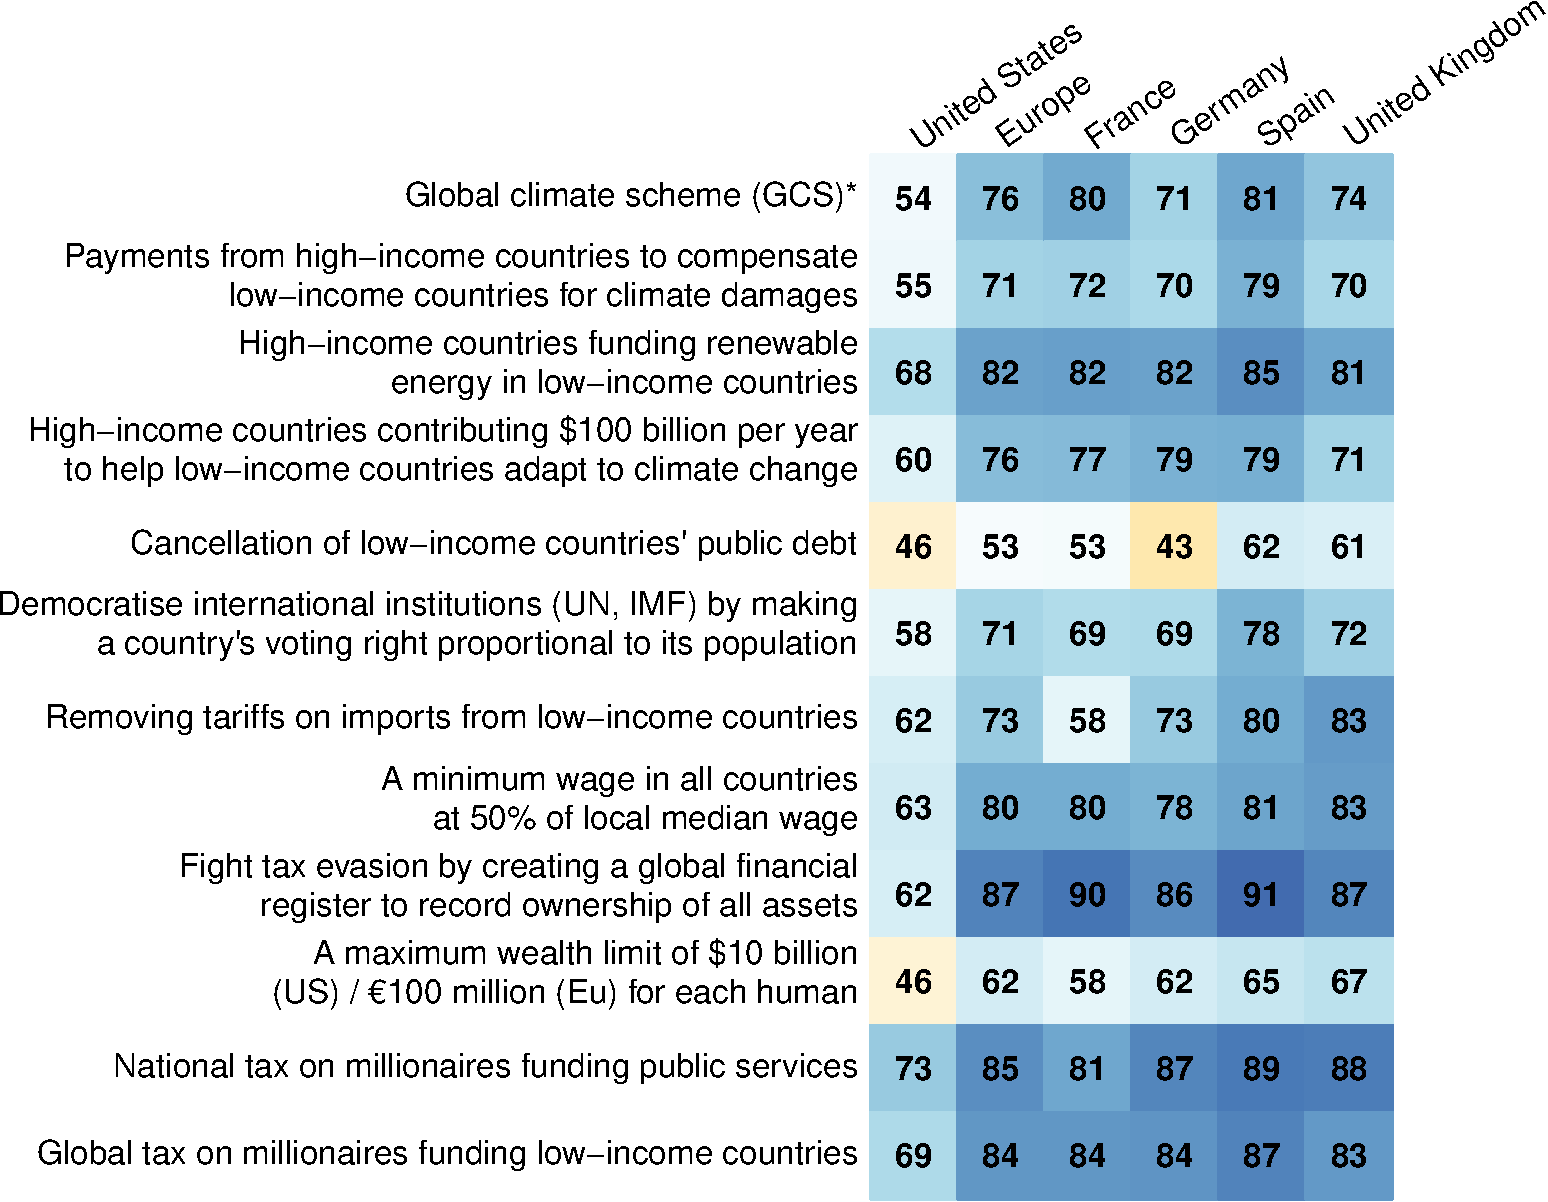
\includegraphics[width=\textwidth]{../figures/country_comparison/support_likert_gcs_share.pdf}}\label{fig:support}
  {\footnotesize Note: The numbers represent the percentage of \textit{somewhat} or \textit{strong support}, after excluding \textit{indifferent} answers. \\
  *Except for the GCS: Share of ``Yes'' in a simple \textit{Yes/No} question. } 
\end{figure} 


\paragraph{Foreign aid}\label{subsubsec:support_foreign_aid} %

We provide respondents with information about the actual amount ``spent on foreign aid to reduce poverty in low-income countries'' relative to their country's government spending and GDP. Less than 16\% of respondents state that their country's foreign aid should be reduced, while 62\% express support for increasing it, including 17\% who support an unconditional increase (Supplementary Figure 5). Among the 45\% who think aid should be increased under certain conditions, we subsequently ask them to specify the conditions they deem necessary (Supplementary Figure 6). The three most commonly selected conditions are: ``we can be sure the aid reaches people in need and money is not diverted'' (73\% chose this condition), ``that recipient countries comply with climate targets and human rights'' (67\%), and ``that other high-income countries also increase their foreign aid'' (48\%). %
On the other hand, respondents who do not wish to increase their country's foreign aid primarily justify their view by prioritizing the well-being of their fellow citizens or by perceiving each country as responsible for its own fate (Supplementary Figure 7). In response to an open-ended question regarding measures high-income countries should take to fight extreme poverty, a large majority of Americans expressed that more help is needed (Supplementary Figure A37). The most commonly suggested form of aid is financial support, closely followed by investments in education. %


We also inquire about the perceived amount of foreign aid. Consistent with prior research (see Supplementary Section A.1.3), most people overestimate the actual amount of foreign aid (Supplementary Figure A18). We then elicit respondents' preferred amount of foreign aid, after randomly presenting them with either the actual amount or no information. Most of the respondents who learn the actual amount choose a bracket at least as high as the actual one, and most of those without the information choose a bracket at least as high as the perceived one (Supplementary Figures A16--A20). 
Finally, we ask a last question to the respondents who received the information. To those who prefer an increase of foreign aid, we ask how they would finance it and find that the preferred source of funding is overwhelmingly higher taxes on the wealthiest (Supplementary Figure A21). To those who prefer a reduction, we ask how they would use the funds becoming available: %
In every country, more people choose higher spending on education or healthcare rather than lower taxes (Supplementary Figure A22). %






\section{Robustness and sincerity of support for the GCS}\label{subsec:robustness_sincerity}

We use several methods to assess the sincerity of the support for the GCS: a list experiment, a real-stake petition, conjoint analyses, and the prioritization of policies. All methods suggest that the support is either completely sincere, or the share of insincere answers is limited. %

\paragraph{List experiment}\label{subsubsec:list_exp} %

We use a list experiment to identify the tacit support for the GCS. To do so, we ask \textit{how many} policies within a list respondents support, and vary the list among respondents. The tacit support is estimated as the difference in the average number of policies supported between two random subsamples, whose list differ only by the inclusion of the GCS.\cite{hainmueller_causal_2014} %
In our case, as shown in Table \ref{tab:list_exp}, the tacit support for the GCS measured through the list experiment is not significantly lower than the direct stated support. %
Hence, we do not find a social desirability bias in our study.


\begin{table} %
  %
  %
  \caption[List experiment: tacit support for the GCS]{Number of supported policies in the list experiment depending on the presence of the Global Climate Scheme (GCS) in the list.%
  }\label{tab:list_exp}
  \makebox[\textwidth][c]{%

\begin{tabular}{@{\extracolsep{5pt}}lccc} 
\\[-1.8ex]\hline 
\hline \\[-1.8ex] 
 & \multicolumn{3}{c}{Number of supported policies} \\ 
\cline{2-4} 
\\[-1.8ex] & All & US & Europe \\ 
\hline \\[-1.8ex] 
 List contains: GCS & 0.624$^{***}$ & 0.524$^{***}$ & 0.724$^{***}$ \\ 
  & (0.028) & (0.041) & (0.036) \\ 
\hline  \\[-1.8ex] \textit{Support for GCS} & 0.65  &  0.542  &  0.757 \\
\textit{Social desirability bias} & \textit{$ -0.026 $} & \textit{$ -0.018 $} & \textit{$ -0.033 $}\\
\textit{80\% C.I. for the bias} & \textit{ $[ -0.06 ; 0.01 ]$ } & \textit{ $[ -0.07 ; 0.01 ]$} & \textit{ $[ -0.08 ; 0.01 ]$}\\
 \hline \\[-1.8ex] 
Constant & 1.317 & 1.147 & 1.486 \\ 
Observations & 6,000 & 3,000 & 3,000 \\ 
R$^{2}$ & 0.089 & 0.065 & 0.125 \\ 
\hline 
\hline \\[-1.8ex] 
\textit{Note:}  & \multicolumn{3}{r}{$^{*}$p$<$0.1; $^{**}$p$<$0.05; $^{***}$p$<$0.01} \\ 
\end{tabular}    }  
  %
\end{table}

\paragraph{Petition}\label{subsubsec:petition}%

We ask respondents whether they are willing to sign a petition in support of either the GCS or NR policy. We inform them that the petition results will be sent to the head of state's office, highlighting the proportion of fellow citizens endorsing the respective scheme. Even when framed as a real-stake petition, both policies continue to receive majority support. In the U.S., we find no significant difference between the support in the real-stake petitions and the simple questions (GCS: $p=.30$; NR: $p=.76$). %
In Europe, the petition leads to a comparable lower support for both the GCS (7 p.p., $p=10^{-5}$) and NR (4 p.p., $p = .008$). While some European respondents are unwilling to sign a petition for policies they are expected to support, this effect is not specific to the GCS, and the overall willingness to sign a real-stake petition remains strong, with 69\% expressing support for the GCS and 67\% for NR.

\paragraph{Conjoint analyses}\label{subsubsec:conjoint}%

In order to assess the public support for the GCS in conjunction with other policies, we conduct a series of conjoint analyses. We ask respondents to make five choices between pairs of political platforms.

The first conjoint analysis suggests that the GCS is supported independently of being complemented by the National Redistribution Scheme and a national climate policy, denoted C.  
For the second analysis, we split the sample into four random branches. %
The outcome is that there is majority support for the GCS and for C, which are seen as neither complement nor substitute (Supplementary Figure A7). A minor share of respondents like a national climate policy and dislike a global one, but as many people prefer a global rather than a national policy; and there is no evidence that implementing NR would increase the support for the GCS.


In the third analysis, we present two random branches of the sample with hypothetical progressive and conservative platforms that differ only by the presence (or not) of the GCS in the progressive platform. Table \ref{tab:conjoint_c} shows that a progressive candidate would not significantly lose voting share by endorsing the GCS in any country, and may even gain 11 p.p. ($p = .005$) in voting intention in France. The effect is also positive at 3 p.p. ($p = .13$) in the U.S., although not significant at the 5\% threshold. %


\begin{table} %
  %
  \caption[Influence of the GCS on electoral prospects]{Preference for a progressive platform depending on whether it includes the GCS or not. (Question 28 in Supplementary Section D) 
  %
Which of these candidates would you vote for? \textit{A; B; None of them} \\
} %
  \makebox[\textwidth][c]{%

\begin{tabular}{@{\extracolsep{5pt}}lcccccc} 
\\[-1.8ex]\hline 
\hline \\[-1.8ex] 
 & \multicolumn{6}{c}{Prefers the Progressive platform} \\ 
\cline{2-7} 
\\[-1.8ex] & All & United States & France & Germany & UK & Spain \\ 
\hline \\[-1.8ex] 
 GCS in Progressive platform & 0.028$^{*}$ & 0.029 & 0.112$^{***}$ & 0.015 & 0.008 & $-$0.015 \\ 
  & (0.014) & (0.022) & (0.041) & (0.033) & (0.040) & (0.038) \\ 
 \hline \\[-1.8ex] 
Constant & 0.623 & 0.604 & 0.55 & 0.7 & 0.551 & 0.775 \\ 
Observations & 5,202 & 2,619 & 605 & 813 & 661 & 504 \\ 
R$^{2}$ & 0.001 & 0.001 & 0.013 & 0.0003 & 0.0001 & 0.0003 \\ 
\hline 
\hline \\[-1.8ex] 
\end{tabular} 
 %
}\label{tab:conjoint_c}
  {\footnotesize \textit{Note:} Simple OLS model. The 14\% of \textit{None of them} answers have been excluded from the regression samples. GCS has no significant influence on them. $^{*}p<0.1$; $^{**} p<0.05$; $^{***} p<0.01$. 
  }
\end{table}
Our last two analyses  make respondents choose between two random platforms. In Europe, respondents are prompted to imagine that a left- or center-left coalition will win the next election and are asked what platform they would prefer that coalition to have campaigned on. In the U.S., the question is framed as a hypothetical duel in a Democratic primary, and asked only to non-Republicans ($n$ = 2,218), i.e. the respondents who choose \textit{Democrat}, \textit{Independent}, \textit{Non-Affiliated} or \textit{Other} for their political affiliation. In the fourth analysis, a policy (or an absence of policy) is randomly drawn for each platform in each of five categories.%
 

In the UK, Germany, and France, a platform is about 9 to 13 p.p. more likely to be preferred if it includes the GCS rather than no foreign policy (Supplementary Figure 8). %
This effect is between 1 and 4 p.p. and no longer significant in the U.S. and in Spain. Moreover, a platform that includes a global tax on millionaires rather than no foreign policy is 5 to 13 percentage points (p.p.) more likely to be preferred in all countries (the effect is significant and at least 9 p.p. in all countries but Spain). 
Similarly, a global democratic assembly on climate change has a significant effect of 8 to 12 p.p. in the U.S., Germany, and France. 
These effects are large, and not far from the effects of the policies most influential on the platforms, which range between 15 and 18 p.p. in most countries (and 27 p.p. in Spain), and all relate to improved public services (in particular healthcare, housing, and education).

The fifth analysis draws random platforms similarly, except that candidate A's platform always contains the GCS while B's includes no foreign policy. In this case, A is chosen by 60\% in Europe %
and 58\% in the U.S. (Supplementary Figure 9). %
In the U.S. for example, our conjoint analyses indicate that a candidate at the Democratic primary would have more chances to obtain the nomination by endorsing the GCS, and this endorsement would not penalize her or him at the presidential election. 






\paragraph{Prioritization}\label{subsubsec:prioritization} %

toward the end of the survey, we ask respondents to allocate 100 points among six randomly selected policies from the previous conjoint analyses, using sliders. The instruction was to distribute the points based on their level of support, with a higher allocation indicating greater support for a policy. %
As a result, the average support across policies is 16.67 points. %
In each country, the GCS ranks in the middle of all policies or above, with an average number of points from 15.4 in the U.S. to 22.9 in Germany (Supplementary Figure A28).%

Interestingly, in Germany, the most prioritized policy is the global tax on millionaires, while the GCS came in as the second most prioritized policy. The global tax on millionaires consistently ranks no lower than fifth position (out of 15 or 17 policies) in every country, garnering an average of 18.3 points in Spain to 22.9 points in Germany.


  

\paragraph{Pros and Cons}\label{subsubsec:pros_cons} %

We survey respondents to gather their perspectives on the pros and cons of the GCS, utilizing either an open-ended or a closed question (Supplementary Figure A8). 
Due to the limited variation in the ratings for each element, the closed question format is inconclusive. %

The open-ended question provides more insights into what people associate with the GCS when prompted to think about it. %
Analyzing keywords in the responses (automatically translated into English), the most frequently mentioned topics are the international aspect and the environment, each appearing in approximately one-quarter of the answers (Supplementary Figure A10). This is followed by discussions on the effects of the GCS on poverty and prices, each mentioned by about one-tenth of the respondents. We also manually classified each answer into different categories (Supplementary Figure A9). This exercise confirms the findings from the automatic search: the environmental benefit of the GCS is the most commonly discussed topic, while obstacles to implementation or agreement on the proposal are relatively infrequently mentioned. %



In the \textit{US2} survey, we divided the sample into four random branches. Two branches were presented the pros and cons questions (either in open or closed format) \textit{before} being asked about their support for the GCS or NR. Another branch received information on the actual level of support for the GCS and NR (estimated in \textit{US1}, see Section \ref{subsec:second_order_beliefs}), and one control group received none of these treatments. %
The objective of this ``pros and cons treatment'' was to simulate a ``campaign effect'',\cite{anderson_can_2023} which refers to the shift in opinion resulting from media coverage of the proposal. To conservatively estimate the effect of a (potentially negative) campaign, we intentionally included more cons (6) than pros (3). Interestingly, the support for the GCS decreased by 11 p.p. after participants viewed a list of its pros and cons. %
Notably, the support also decreased by 7 p.p. after participants were asked to consider the pros and cons in an open-ended question. Although support remains significant, %
these results suggest that the public success of the GCS would be sensitive to the content of the debate about it, and subject to the discourse adopted by interest groups.



\section{Universalistic values}\label{subsec:universalistic}

To better understand people's support for specific policies, we also elicit underlying values. %
When we ask participants which group they defend when they vote, %
20\% choose ``sentient beings (humans and animals),'' 22\% choose ``humans,'' 33\% select their fellow citizens (or ``Europeans''), 15\% choose ``My family and myself,'' and the remaining 10\% choose another group (mainly ``My State or region'' or ``People sharing my culture or religion''). 
Notably, a majority of left-wing choose ``humans'' or ``sentient beings'' 
(see Supplementary Figure A38 for main attitudes by vote).%

When asked what their country's diplomats should defend in international climate negotiations, only 11\% prefer their country's ``interests, even if it goes against global justice'' (Supplementary Figure A27). In contrast, 30\% prefer global justice (with or without consideration of national interests), and the bulk of respondents (38\%) prefer their country's ``interests, to the extent it respects global justice.''

Furthermore, when we ask participants to assess the extent to which climate change, global poverty, and inequality in their country are issues, climate change is generally viewed as the most significant problem (with a mean score of 0.59 after recoding answers between -2 and 2). This is followed by global poverty (0.42) and national inequality (0.37). %

Finally, we conduct a lottery experiment to elicit universalistic values. Respondents were automatically enrolled in a lottery with a \$100 prize and had to choose the proportion of the prize they would keep for themselves versus give to a person living in poverty. The charity donation is directed either to an African individual or a fellow citizen, depending on the respondent's random assignment. In Europe, we observe no significant variation in the willingness to donate based on the recipient's origin, while in the U.S., the donations to Africans are 3 p.p. lower (with an average donation of 34\%). Moreover, the slightly lower donations to Africans are entirely driven by Trump voters and non-voters (Supplementary Table A2).


\section{Second-order Beliefs}\label{subsec:second_order_beliefs}
To explain the strong support for the GCS despite its absence from political platforms and public debate, we hypothesized pluralistic ignorance, i.e. that the public and policymakers mistakenly perceive the GCS as unpopular. As a result, individuals might conceal their support for such globally redistributive policies, believing that advocating for them would be futile. However, the evidence for pluralistic ignorance is limited based on an incentivized question about perceived support (Supplementary Figure 10).

Beliefs about the level of support for the GCS are fairly accurate for U.S. subjects. The mean perceived support is 52\% (with quartiles of 36\%, 52\%, and 68\%), which closely aligns with the actual support of 53\%. Europeans, on the other hand, underestimate the support by 17 p.p. Nonetheless, 65\% of them correctly estimate that the GCS garners majority support, and the mean perceived support is 59\% (and quartiles of 43\%, 61\%, and 74\%), compared to the actual support of 76\%. Second-order beliefs are equally accurate for NR in the U.S. and similarly underestimated in Europe. %
Finally, consistent with U.S. subjects accurately perceiving the levels of support for the GCS or NR, providing information on the actual level had no significant effect on their support in the \textit{US2} survey. %



\section{Discussion} %
Our point of departure are recent surveys %
in 20 of the largest countries, %
as they reveal robust majority support for global redistributive and climate policies, even in high-income countries that would financially lose from them.\cite{dechezlepretre_fighting_2022} The results from %
complementary surveys conducted in the U.S. and four European countries %
reinforce these findings. We find strong support for global taxes on the wealthiest individuals, as well as majority support for our main policy of interest -- the Global Climate Scheme (GCS). The GCS encompasses carbon pricing at a global level through an emissions trading system, accompanied by a global basic income funded by the scheme's revenues. Additional experiments, such as a list experiment and a real-stake petition, demonstrate that the support for the GCS is real. 
Such genuine support is further substantiated by the prioritization of the GCS over prominent national climate policies and aligned with a significant portion of the population holding universalistic values rather than nationalistic or egoistic ones. Moreover, the conjoint analyses indicate that a progressive candidate would not lose voting shares by endorsing the GCS, and may even gain 11 p.p. in voting shares in France. Similarly, a candidate endorsing the GCS would gain votes in a U.S. Democratic primary, while in Europe, a progressive platform that includes the GCS would be preferred over one that does not.


What could explain the gap between sincere support of citizens and the scarce mention in public debate? First, there may be pluralistic ignorance \textit{among policymakers} regarding universalistic values, support for global redistribution, or the electoral advantage of endorsing it. Second, people or policymakers may believe that globally redistributive policies are technically impossible or politically infeasible in some key (potentially foreign) countries. %
Third, political discourse centrally happens at the national level, shaped by national media and institutions such as voting. 
National framing by political voices may create biases and suppress universalistic values. Uncovering evidence to support these hypotheses could %
draw attention to global policies in the public debate and contribute to their increased prominence.%







\begin{methods}  %
  %
\fakesection{Methods}\label{sec:methods}
\subsection{Data collection.} %

The paper utilizes two sets of surveys: the \textit{Global} survey and the \textit{Complementary} surveys. The \textit{Complementary} surveys consist of two U.S. surveys, \textit{US1} and \textit{US2}, and one European survey, \textit{Eu}. The \textit{Global} survey was conducted from March 2021 to March 2022 on 40,680 respondents from 20 countries (with 1,465 to 2,488 respondents per country). \textit{US1} collected responses from 3,000 participants between January and March 2023, while \textit{US2} gathered data from 2,000 respondents between March and April 2023. \textit{Eu} included 3,000 participants and was conducted from February to March 2023. We used the survey companies \emph{Dynata} and \emph{Respondi}. To ensure representative samples, we employed stratified quotas based on gender, age (5 brackets), income (4), region (4), and education level (3), as well as ethnicity (3) for the U.S. We also incorporated survey weights throughout the analysis to account for any remaining imbalances. These weights were constructed using the quota variables as well as the degree of urbanity, and trimmed between 0.25 and 4. By applying weights, the results are fully representative of the respective countries. Results at the European level apply different weights which ensure  representativeness of the combined four European countries. 
Supplementary Section G confirm that our samples closely match population frequencies in high-income countries. In middle-income countries, the samples are only representative of the online population (young, graduated and urban people are over-represented). %


\subsection{\small Data quality.} %
The median duration is 28 minutes for the \textit{Global} survey, 14 min for \textit{US1}, 11 min for \textit{US2}, and 20 min for \textit{Eu}. To ensure the best possible data quality, we exclude respondents who fail an attention test or rush through the survey (i.e., answer in less than 11.5 minutes in the \textit{Global} survey, 4 minutes in \textit{US1} or \textit{US2}, 6 minutes in \textit{Eu}). %



\subsection{\small Questionnaires and raw results.} %
The questionnaire and raw results of the \textit{Global} survey can be found in the Appendix of the companion paper Dechezleprêtre et al. (2022).\cite{dechezlepretre_fighting_2022} %
The raw results are reported in Supplementary Section B %
while the surveys' structures and questionnaires are given in Supplementary Sections C and D. The questionnaires are the same as the ones given \textit{ex ante} in the registration plan (\href{https://osf.io/fy6gd}{osf.io/fy6gd}).


\subsection{\small Incentives.} %
To encourage accurate and truthful responses, several questions of the \textit{US1} survey use incentives. For each of the three comprehension questions that follow the policy descriptions, we randomly select and reward three respondents who provide correct answers with a \$50 gift certificate. Similarly, for questions involving estimating support shares for the GCS and NR, three participants with the closest guesses to the actual values receive a \$50 gift certificate. In the donation lottery question, we randomly select one respondent and split the \$100 prize between the NGO GiveDirectly and the winner according to the winner's choice. In total, our incentives scheme distributes gift certificates (and donations) for a value of \$850. Finally, respondents have an incentive to answer truthfully to the petition question, as they are aware that the results for that question (the share of respondents supporting the policy) will be transmitted to the head of state's office.






\subsection{Support for the GCS} The 95\% confidence intervals are $[52.4\%, 55.9\%]$ in the U.S. and $[74.2\%, 77.2\%]$ in Europe. The average support is computed with survey weights, employing weights based on quota variables, which exclude vote. Another method to reweigh the raw results involves running a regression of the support for the GCS on sociodemographic characteristics (including vote) and multiplying each coefficient by the population frequencies. This alternative approach yields similar figures: 76\% in Europe and 52\% or 53\% in the U.S. (depending on whether individuals who did not disclose their vote are classified as non-voters or excluded). Notably, the average support excluding non-voters is 54\% in the U.S. 

Though the level of support for the GCS is significantly lower in swing States (at 51\%) that are key to win U.S. elections, the electoral effect of endorsing the GCS remains non-significantly different from zero (at +1.2 p.p.) in these States. Note that we define swing states as the 8 states with less than 5 p.p. margin of victory in the 2020 election (MI, NV, PA, WI, AZ, GA, NC, FL). The results are robust to using the 3 p.p. threshold (that excludes FL) instead. 

\subsection{Global wealth tax estimates}
A 2\% tax on net wealth exceeding \$5 million would annually raise \$816 billion, leaving unaffected 99.9\% of the world population. More specifically, it would collect \euro{}5 billion in Spain, \euro{}16 billion in France, £20 billion in the UK, \euro{}44 billion in Germany, \$430 billion in the U.S., and \$1 billion collectively in all low-income countries (28 countries, home to 700 million people). These Figures come from the \href{https://wid.world/world-wealth-tax-simulator/}{WID wealth tax simulator}.\cite{chancel_world_2022}

\subsection{List experiment}
We utilize the difference-in-means estimator, and confidence intervals are computed using Monte Carlo simulation with the R package \textit{list}.\cite{imai_multivariate_2011}

\subsection{Petition}
Paired weighted \textit{t}-tests are conducted to test the equality in support for a policy among respondents who were questioned about the policy in the petition.

\subsection{Conjoint analysis}
The effects reported in the fourth analyses are the Average Marginal Component Effects.\cite{hainmueller_causal_2014} The policies studied are progressive policies prominent in the country. Except for the category \textit{foreign policy}, which features the GCS 42\% of the time, they are drawn uniformly.

\subsection{Pros and cons}
Surprisingly, the support for National Redistribution also decreased by 7 p.p. following the closed question about the GCS. This suggests that some individuals may lack attention and confuse the two policies, or that contemplating the pros and cons alters the mood of some people, moving them away from their initial positive impression.

\subsection{Sources}
Detailed sources for the questionnaires and the figures are given in the \href{https://github.com/bixiou/international_attitudes_toward_global_policies/raw/main/questionnaire/specificities.xlsx}{Supplementary Spreadsheet}.

\subsection{\normalsize Data and code availability}

All data and code of the \textit{Complementary} surveys as well as figures of the paper are available on \href{https://github.com/bixiou/international_attitudes_toward_global_policies}{github.com/bixiou/international\_attitudes\_toward\_global\_policies}. Data and code for the \textit{Global} survey will be made public upon publication.

\end{methods} %

\fakesection{Bibliography}\label{sec:bib}
\bibliographystyle{naturemag_noURL} %
\bibliography{global_tax_attitudes}



\begin{addendum} %
 \item We are grateful for financial support from the University of Amsterdam and TU Berlin. Mattauch also thanks the Robert Bosch Foundation. We are grateful for financial support from the OECD, the French Ministry of Foreign Affairs, the French Conseil d'Analyse Economique and the Spanish Ministry for the Ecological Transition and Demographic Challenge. We also acknowledge support from the Grantham Foundation for the Protection of the Environment and the Economic and Social Research Council through the Centre for Climate Change Economics and Policy. 
We thank Antoine Dechezleprêtre, Tobias Kruse, Bluebery Planterose, Ana Sanchez Chico, and Stefanie Stantcheva for their invaluable inputs for the project. We thank Antonio Bento, Dietmar Fehr, and Auriane Meilland for feedback. We further thank Jakob Niemann, Laura Schepp, Martín Fernández-Sánchez, Samuel Gervais, Samuel Haddad, and Guadalupe Manzo for assistance. 
 \item[Registration] The project %
 was preregistered in the Open Science Foundation registry (osf.io/fy6gd).
 \item[Competing Interests] Fabre declares that he also serves as president of Global Redistribution Advocates.
\item[JEL codes] P48, Q58, H23, Q54.
\item[Keywords] Climate change, global policies, cap-and-trade, perceptions, survey, inequality, wealth tax.
 \item[Correspondence] Correspondence and requests for materials
should be addressed to Adrien Fabre~(email: adrien.fabre@cnrs.fr).
\end{addendum}



\end{document}
